\section{Experiments \& Results}

% In this section, we describe the experiments and results supporting the contributions outlined in the introduction. 
\begin{figure*}[h!]
\centering
    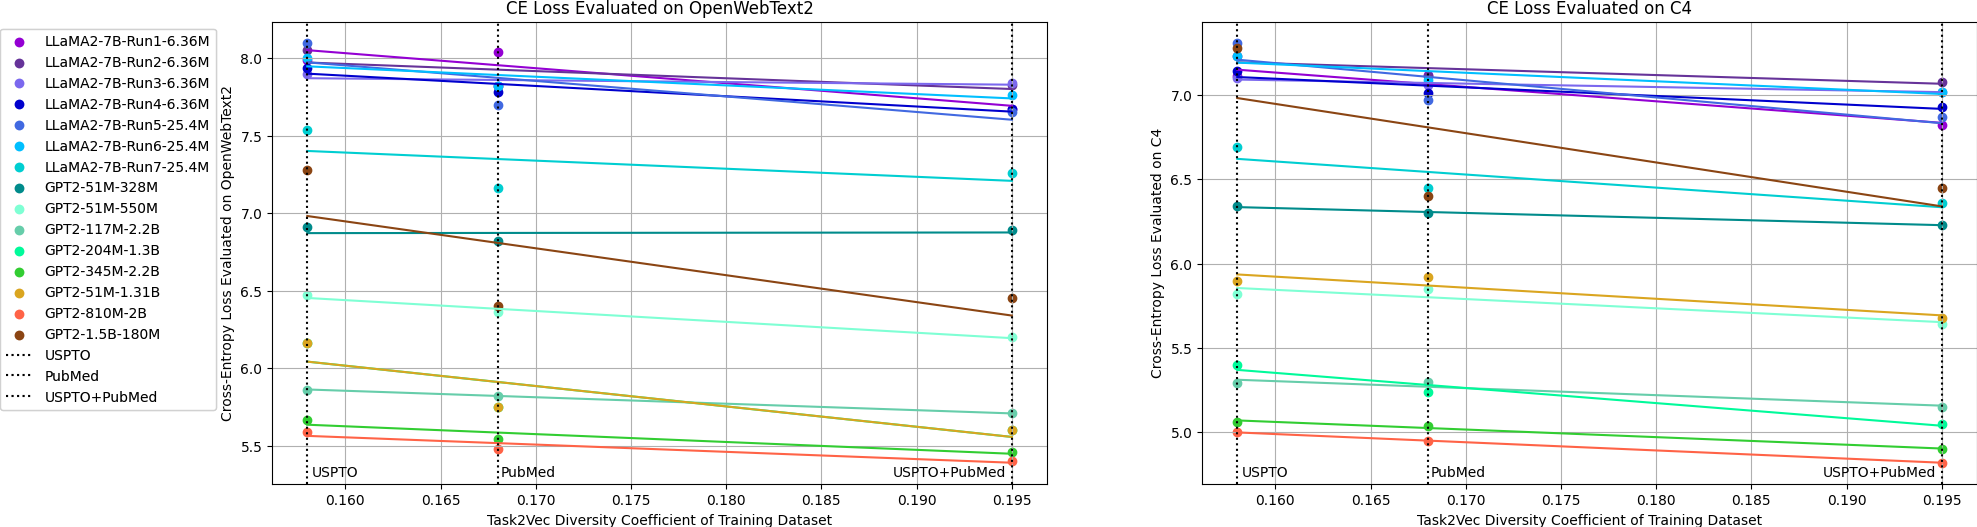
\includegraphics[width=\textwidth]{plots/div_vs_val_ce_2.png}
  \caption{
  \textbf{Pre-training on datasets with higher diversity coefficients leads to better evaluation performance on diverse datasets.} 
  Legends are formatted ``Model Type-Number of Parameters-Number of Tokens trained on". 
  The models were evaluated on the validation sets. 
  The diversity of the pre-training datasets increase from $0.158$, to $0.168$, to $0.195$. 
  Models are evaluated on the validation split of the given evaluation dataset (given in each plot's title). 
All models of the same run (i.e. same color) are trained on the same number of tokens and the same hyperparameters, minimizing cofounding factors. 
  }
  \label{fig:div_vs_val_ce}
\end{figure*}
% Finally, we conduct a comprehensive set of controlled \textit{interventional} experiments with GPT-2 and LLaMAv2 that demonstrates the diversity coefficient of pre-training data is a meaningful driver of downstream model evaluation performance---totaling 33 models trained of various sizes (54M  to 7B).

\subsection{Pre-training in Higher Diversity Leads to Better Evaluation Performance}
Next, we highlight one of our main empirical results, showing that pre-training from scratch on data sets of \textbf{increasing formal diversity} leads to \textbf{better evaluation performance} on the validation set. 
We want to emphasize that our results are \textit{interventional and not correlative}---
i.e., we intervene by constructing pre-training data sets of increasing diversity, train the models from scratch on these (controlling tokens), and finally demonstrate performance improves.  

\textbf{Experiments: } 
We computed the formal diversity coefficient (described in section \ref{body:div_coeff_natural_lang}) of three publicly available datasets (USPTO, PubMed, and the combination of USPTO+PubMed) with diversity values of 0.158, 0.168, and 0.195 respectively. 
We then pre-trained GPT2s \citep{gpt2} models of size 51M, 117M, 204M, 345M, 810M, 1.5B parameters and LLaMAv2 7B \citep{llamav2} from scratch. 
To ensure that the diversity of the dataset is the primary factor driving our results, we train all models using a fixed number of tokens and the same hyperparameters across the same experiment. 
An experiment is considered to be the triplet of models trained with the USPTO, PubMed, and USPTO+PubMed. 
The 51M model is trained on 550M tokens, the 117M model is trained on 2.2B tokens, the 204M model is trained on 1.3B tokens, the 345M model is trained on 2.2B tokens, the 810M model is trained on 2B tokens, and the 1.5B model is trained on 180M tokens. 
The LaMMAv2 7B model is trained on 6.36M tokens. 
For training runs with combined datasets, each batch has interleaved examples from both datasets with equal mixing proportions. 

\textbf{Results: }
Figure \ref{fig:div_vs_val_ce} demonstrates that as the diversity coefficient of the pre-training dataset increases, the evaluation performance improves. 
This key result follows because the cross-entropy loss on the validation falls on all 15 runs in \ref{fig:div_vs_val_ce}. 
We evaluated on the validation set of C4 and OpenWebText2 which have diversity coefficients of 0.237 and 0.222. 
We deliberately avoided selecting the Pile in order to minimize contamination issues that could potentially confound our results. 
We also deliberately selected dataset with high diversity because the conjecture is that diverse pre-training datasets help the most on diverse general evaluation benchmarks. 
Our results also have positive average $R^2$ values of approximately 0.79 for OpenWebText2, 0.82 for C4 when including all 8 GPT-2 experiments---all trained for over 150M tokens, and most over 1B tokens---and similar $R^2$ values when also including all remaining LLaMA2 experiments (larger models trained on fewer tokens). 
% We also fined that aligned datasets helped. 
% TODO: do low div data set?

\subsection{Diversity Coefficients of Pre-training Data shows LLMs are Pre-trained on Formally Highly Diverse Data}

\textbf{Experiments:} 
We evaluate the diversity coefficient and cross diversity coefficient (both described in section \ref{body:div_coeff_natural_lang}) of ten publicly available LLM pre-training datasets (described in section \ref{appendix:datasets}).
% We evaluate the cross diversity coefficient (described in section \ref{cross_div_coeff}) of eight publicly available LLM pre-training datasets (described in section \ref{section:datasets}).
% We also compute the diversity coefficient (described in section \ref{div_coeff}) of ten publicly available LLM pre-training data sets (described in section \ref{section:datasets}).
We also compute the diversity and cross diversity coefficients of two concatenated datasets: 
1) C4 and WikiText-103, and 
2) five sub-datasets of The Pile: Pile-CC, HackerNews, NIH ExPorter, PubMed, and USPTO (Appendix \ref{appendix:concat_datasets}).
In addition, we compute our conceptually well-motivated lower and upper bounds on the diversity coefficient (section \ref{method_ub_lb}).

\textbf{Results:}
Table \ref{tab:div} reports the aforementioned diversity and cross diversity coefficients. 
The key observations from our results are:
\begin{itemize}
    \item The cross diversity coefficients of pre-training datasets tend to be \textbf{3-5 times greater than the theoretical lower bound and, on average, half the upper bound.} 
    Prominently, C4, The Pile, and Pile-CC exhibit the highest diversity coefficients (0.23 - 0.25). This aligns with intuition, as these are very large, web-crawl-based, internet-scale datasets. 
    \item The diversity coefficients of pre-training datasets tend to be \textbf{2.7-4.76 times greater than the theoretical lower bound and, on average, half the upper bound.}
    As expected, this is slightly lower than the cross diversity coefficient because the cross diversity coefficient compares batch embeddings from different, disjoint datasets.
    % \item The measured diversity of Pile-CC is higher than that of C4, indicating a potentially more stringent preprocessing method applied to the Common Crawl corpus for Pile-CC, which contributes to enhanced data diversity.
    % \item Three sub-datasets of The Pile---NIH ExPorter, PubMed Abstracts, and USPTO---show relatively low diversity (0.15 - 0.17), less than half of the upper bound (0.4). 
    % These datasets are curated from specialized fields with regular formats and topics, which may account for this observation. 
    % % For instance, patent backgrounds in USPTO may share similar formatting and semantics as do abstracts in NIH ExPorter or PubMed Abstracts.
    % \item However, we observe that Pile-CC and HackerNews have higher diversity (.20 - .25), which may be attributed to their coverage of a broad range of topics. 
    % % Among these, Pile-CC exhibits higher diversity, in line with its heterogeneous content composition.
\end{itemize}


\begin{figure*}[h!]
\centering
    \includegraphics[width=0.35\columnwidth]{plots/histogram_C4andwt_400tasks_bs512.png}
    \includegraphics[width=0.35\columnwidth]{plots/violinplot_C4andwt_400tasks_bs512.png}
    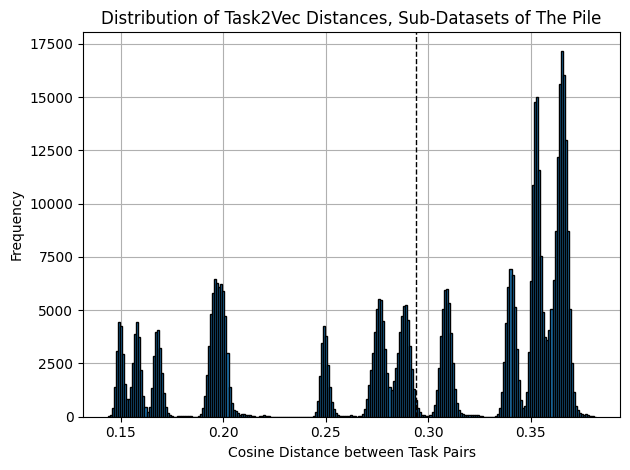
\includegraphics[width=0.35\columnwidth]{plots/histogram_all_thepile_subds.png}
    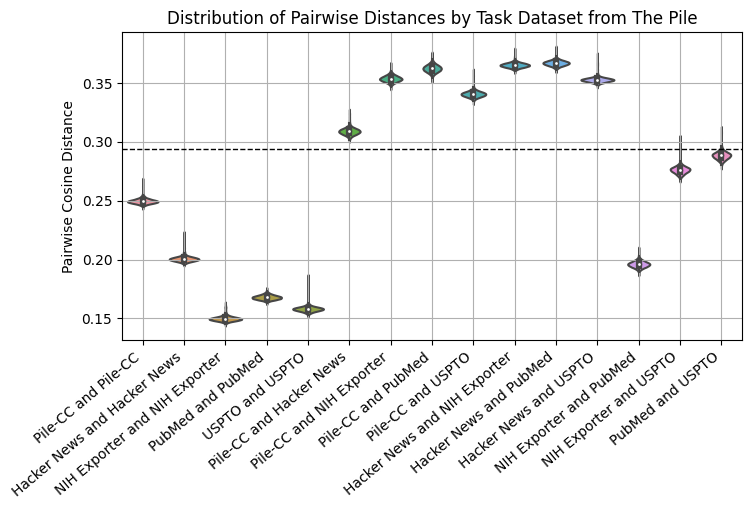
\includegraphics[width=0.35\columnwidth]{plots/violin_plot_all_thepile_subds.png}
  \caption{
  \textbf{Distribution of pairwise batch distances reflects conceptual and semantic dataset properties, therefore increasing trust in the diversity and cross diversity coefficient.} 
  Pairwise task distances from the concatenated C4 and WikiText-103 dataset (top) and concatenated five sub-datasets of The Pile (bottom) take on a multi-modal form according to dataset comparisons. 
  Pairwise distances are segmented by source datasets for each pair of batches (right), where each sub-distribution corresponds to a mode from the histograms (left).
  Dotted lines denote the cross diversity coefficient of the concatenated C4 and WikiText-103 dataset (top) and concatenation of five sub-datasets of The Pile (bottom). 
  These results show that combining batches from two different datasets computes a higher cross diversity, as expected. 
  Therefore, these results align with human intuition, increasing the confidence in the diversity and cross diversity coefficients as diversity metrics.
  % that combining datasets from different sources increases the overall data diversity.
  }
  % The first five violins show distributions of pairs of batches from the same dataset. The remaining violins show distance distributions between pairs where no two batches in a pair are from the same dataset. 
  \label{fig:concat_div}
\end{figure*}


\subsection{Concatenation of Datasets of Different Sources Produces Higher Measured Diversity}

\textbf{Experiments:} 
To show that the concatenation of different datasets produces high diversity datasets, we measure the cross diversity coefficient of C4 plus WikiText-103, as well as of the five sub-datasets of The Pile in Table \ref{tab:div}.
To understand the source of this increased diversity, we plot in Figure \ref{fig:concat_div} the Task2Vec (cosine) distances between batches from individual datasets and distances of batches from the different datasets.

\textbf{Results:}
Our key observations are:
\begin{itemize}
    \item The cross diversity coefficient for the C4 and WikiText-103 concatenated dataset is 0.2711, about +0.03-0.05 higher than that of each individual dataset.
    \item The cross diversity coefficient for the concatenation of the five sub-datasets of the Pile is 0.2939 (Table \ref{tab:div}), which is about +0.04-0.1 (Figure \ref{fig:concat_div}) that of each individual dataset.
    % \item The concatenation of the five sub-datasets of The Pile achieves the highest diversity coefficient in Table \ref{tab:div}. 
\end{itemize}
This increase in diversity occurs because concatenating datasets produces higher pairwise Task2Vec distances between batches from different datasets (see Figure \ref{fig:concat_div}).
% This results in a higher diversity coefficient, since the coefficient is an average of all pairwise Task2Vec distances.
Note that, this aligns with human intuition that combining data from heterogeneous sources increases the overall diversity of the data.

\subsection{Distribution of Pairwise Batch Distances Reflects Conceptual and Semantic Dataset Information}
To increase our confidence in the diversity and cross diversity coefficient as diversity metrics, we study distributions of the Task2Vec (cosine) distances used to compute the coefficient.
% In particular, we study if the grouping of these distances align with human conceptual and semantic understanding.
% should we include the word intuitive? In particular, we study if the grouping of these distances align with human intuitive conceptual and semantic understanding.
We examine the alignment of the grouping of these distances with (human) conceptual and semantic understanding in Figure \ref{fig:concat_div}.

\textbf{Experiments:}
% We reason about relative pairwise distance distributions using knowledge of the data sources and composition. 
We analyze Task2Vec (cosine) distances between batches from five sub-datasets of The Pile.
We compare distances between batches of individual sub-datasets and distances across different sub-datasets.
% We show the resulting histograms and violin plots in Figure \ref{fig:concat_div}. 
% We also segment these distances between batches across C4 and WikiText-103 in Figure \ref{fig:concat_div}.
% todo, report that we computed the dist hist of C4 wikitext-103 hist for 8 pager, then add \item bellow for it

\textbf{Results:}
Our key observations are:
\begin{itemize}
    % 1. histograms have modes related to number of datasets.
    \item Figure \ref{fig:concat_div} (top, left) shows 3 modes. 
    We confirm that the modes correspond to pairings of datasets in Figure \ref{fig:concat_div} (top, right). 
    For instance, the right-most mode, corresponding to distances with values higher than the cross diversity coefficient, consists of pairwise distances between C4 and WikiText-103 batches. 
    This confirms intuitive properties we'd expect, i.e. we'd expect 3 modes given 2 datasets ($C^2_2 + 2 = 3$).
    \item Similarly to the preceding point, Figure \ref{fig:concat_div} (bottom, left) shows 15 modes, which is exactly the number expected in enumerating all possible pairs of batches from 5 datasets.\footnote{Given a 5 by 5 distance matrix, we'd expect the lower triangular portion plus the diagonal to be the number of pairings, so $C^5_2 + 5 = 15$.}
    Due to overlaps in distance values we only see 11 modes in the Figure \ref{fig:concat_div} (bottom, right).
    % \item We also observe that the combined datasets have an increased diversity coefficient compared to the individual data sets. 
    % We outlined this in the previous section, but we underscore it here to emphasize this semantic property.
    % \item We expect pairings of unrelated datasets to have higher cross diversity compared to pairings of related datasets.
    % We observe this in Figure \ref{fig:concat_div} (right).
    % For the concatenated dataset of C4 and WikiText-103, the distribution of pairwise distances where one batch is from C4 and one is from WikiText-103 (right-most violin) is higher than that of individual datasets.
    % For the concatenated sub-datasets of The Pile, the violin plots for combinations of conceptually unrelated datasets group above the dotted line (e.g. Hacker News and PubMed), while the violin plots of technical subjects written similarly
    % \footnote{e.g. NIH ExPorter and PubMed Abstracts both contain academic, medicine-focused writing, and have the lowest distances (third violin from the right) among combinations of different datasets.} 
    % are below the dotted line (e.g. PubMed and USPTO).
    % Note however that all combined cross diversities always increased after a concatenation.
% 3. In particular, unrelated datasets are above dotted line while related data sets (technical & HNws + Pile-CC) are bellow the dotted line.
    %\item in ref to above C4, wikitext-103 add observations here, 3 modes mainly. 
    % \item We expect Pile-CC and HackerNews to cover the most diverse topics since they are broad web-scale datasets, unlike the remaining which are technical in nature.
    % Therefore, we anticipate 
    % 1) these two to have the highest individual diversities, as shown in the first two violin plots in Figure \ref{fig:concat_div}, and
    % 2) to have the highest increase when concatenated with other datasets, as shown in the 6th to the 12th violin plots when counting from the left, in Figure \ref{fig:concat_div}.
    % \item Distances between batches from Pile-CC and HackerNews (sixth violin from the left) are the lowest among pairwise distances of concatenated datasets above the cross diversity coefficient.
    % This aligns with human conceptual intuition because the Pile-CC and HackerNews are the most similar in those sub-datasets, since they are both web-scale datasets. 
\end{itemize}
These findings build trust in the cross diversity coefficient as a dataset diversity metric, since the coefficient and underlying Task2Vec distances of batches behave in interpretable ways that align with human intuition. Since the diversity coefficient uses the same computational backbone as cross diversity, these findings also build trust in the diversity coefficient. %, which can be applied with more versatility. %, unlike cross diversity, can %be applied to unioned datasets %without the need to segment the overall dataset into sub-datasets.

% Pairwise distances distributed above the diversity coefficient (dotted line) have one task from Pile-CC or HackerNews and one from another sub-dataset. 
% This matches our reasoning that Pile-CC and HackerNews cover diverse topics as web-scale datasets, and therefore, each have the highest individual diversity coefficients out of the five sub-datasets of The Pile. 
% Distances between a task from Pile-CC and a task from HackerNews (sixth violin from the left) are distributed the lowest among pairwise distances above the diversity coefficient, which corresponds to the same line of reasoning.

\subsection{Diversity Coefficient Captures LLM Pre-training Data Distributional Properties} \label{body:ginc}
To instill further confidence in the diversity coefficient, we perform a correlation analysis with data distributional properties on the GINC dataset synthetic language dataset \cite{ginc}.
GINC generates sequences by modeling how real documents are generated given a fixed number of latent document concepts through a mixture of Hidden Markov Models (HMM), where each HHM has a latent concept that models document statistics, e.g. wiki bio.
Further details on GINC can be found in section \ref{appendix:ginc}.

\textbf{Experiments:}
Given that each GINC dataset is a mixture of HMMs with a fixed number of latent concepts (1-10,000), we plot how the diversity coefficient varies as the number of latent concepts increases for each dataset.
We plot this in Figure \ref{fig:div_rsquared} (top) and fit a curve for GINC datasets with fixed vocabulary sizes of 50 and 150.
Then we fix the number of latent concepts at 5 and 5000 and similarly plot how increasing the vocabulary size for the GINC dataset (50-10,000 unique tokens) increases the diversity coefficient.
We plot this in Figure \ref{fig:div_rsquared} (bottom) and fit a curve for GINC datasets with 5 latent concepts and 5000 latent concepts.

\textbf{Results:}
Our observations are as follows:
\begin{itemize}
    \item \textbf{Diversity coefficient increases with greater number of latent concepts.} 
    Figure \ref{fig:div_rsquared} (top) shows adding more latent concepts increases the diversity coefficient with diminishing returns.
    We hypothesize that additional latent concepts introduce new and varied document-level statistics, resulting in an increase in the diversity coefficient.
    The $R^2$ is high, with values 0.952 and 0.898.
    \item The diversity coefficient eventually saturates as more latent concepts are added. 
    We hypothesize this is due to the small size of a synthetic data set vs. a real one.
    % We hypothesize this may be due to marginal increases in variation from increased overlap, 
    % e.g. wiki bios and autobiographical web pages may have syntactical and semantic similarities.
    \item \textbf{Diversity coefficient increases with larger vocabularies.}
    Figure \ref{fig:div_rsquared} (bottom) shows the measured diversity coefficient increases at a seemingly exponential pace for larger vocab sizes.
    The $R^2$ is high with values 0.993 and 0.984.
    % \item We hypothesize the growth might be exponential because scaling the number of tokens produces a more diverse dataset by vastly increasing the number of ways to represent any sequence.
    % More formally, given a sequence $x$ of length $T_x$ and vocab size $|V|$, the number of ways to represent that sequence is approximately $|V|^{T_x}$.
    % Therefore, as $|V|$ increases, the growth rate of the exponential increases. 
\end{itemize}
These results show the diversity coefficient successfully captures different distributional sources of variation of the data.

\begin{figure*}[h]
    \centering
    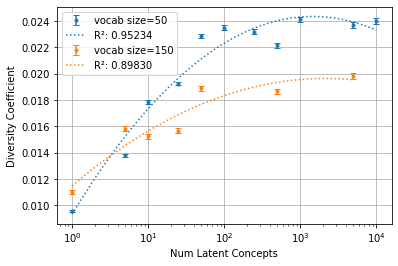
\includegraphics[width=0.4\linewidth]{plots/div_nlatents_rsquared.png}
    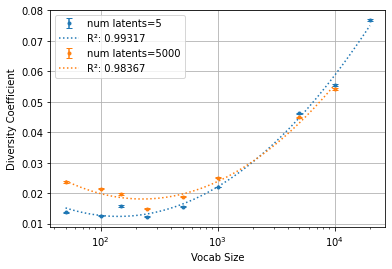
\includegraphics[width=0.4\linewidth]{plots/div_vocab_rsquared.png}
  \caption{\textbf{Diversity coefficient of GINC datasets with varying number of latent concepts and vocab sizes shows the diversity coefficient behaves as expected.} 
  The diversity coefficient increases and saturates with an increasing number of latent concepts (top) and exponentially increases with increasing vocab size (bottom). 
  This implies that increases in the measured diversity coefficient correspond to changes in LM pre-training data distributional properties that intuitively enable more diverse data. } 
  %  $R^2$ measures how well the curves fit the observed values.
  \label{fig:div_rsquared}
\end{figure*}


%%%%%%%%%%%%%%%%%%%%%%%%%%%%%%%%%%%%%%%%%%%%%%%%%%%%%%%%%%%%%%%%%%%%%%%%%%%%%%%%%%%%%%%%
